\documentclass[letterpaper,12pt]{book}
\nonstopmode

%%%%%%%%%%%%%%%%%%%%%%%%%%%%%%%%%%%%%%%%%%%%%%%%%%%%%%%%%%%%%%%%%%%%%%%
% Packages
%%%%%%%%%%%%%%%%%%%%%%%%%%%%%%%%%%%%%%%%%%%%%%%%%%%%%%%%%%%%%%%%%%%%%%%
% Formatting
\usepackage[headheight=35pt,hmargin=0.5in,vmargin=0.75in]{geometry}
\usepackage{amsmath,amsthm,amssymb}
\usepackage{fancyhdr, parskip}
\usepackage{listings}
\usepackage{placeins}

% Tables and Figures
\usepackage{graphicx}
\usepackage{caption}
\usepackage{subcaption}
\usepackage{multirow}
\usepackage{xltabular}
\usepackage[framemethod=TikZ]{mdframed}

% Citations
\usepackage{cite}

% Additional Info
\usepackage{lastpage}

% Hyperref Should remain the last import in most circumstances
\usepackage{hyperref}
  \hypersetup{
    colorlinks=true,
    linkcolor=blue,
    filecolor=magenta
    urlcolor=cyan
  }

%%%%%%%%%%%%%%%%%%%%%%%%%%%%%%%%%%%%%%%%%%%%%%%%%%%%%%%%%%%%%%%%%%%%%%%
% Title Page Information
%%%%%%%%%%%%%%%%%%%%%%%%%%%%%%%%%%%%%%%%%%%%%%%%%%%%%%%%%%%%%%%%%%%%%%%
\title{Scouts BSA Programming Project Guide}
\author{
  Benjamin Davis [\href{mailto:benjamin.j.davis96@gmail.com}{benjamin.j.davis96@gmail.com}]
}
\date{Copyright \copyright\ \the\year\ Benjamin Davis}

%%%%%%%%%%%%%%%%%%%%%%%%%%%%%%%%%%%%%%%%%%%%%%%%%%%%%%%%%%%%%%%%%%%%%%%
% Header & Footer Information
%%%%%%%%%%%%%%%%%%%%%%%%%%%%%%%%%%%%%%%%%%%%%%%%%%%%%%%%%%%%%%%%%%%%%%%
\fancypagestyle{plain} {
  \fancyhf{}
  \fancyhead[L]{BSA Programming MB}
  \fancyhead[R]{\leftmark}
  \fancyfoot[R]{\thepage}
}

\fancypagestyle{simple}{
  \fancyhf{}
}

%%%%%%%%%%%%%%%%%%%%%%%%%%%%%%%%%%%%%%%%%%%%%%%%%%%%%%%%%%%%%%%%%%%%%%%
% Graphics Information
%%%%%%%%%%%%%%%%%%%%%%%%%%%%%%%%%%%%%%%%%%%%%%%%%%%%%%%%%%%%%%%%%%%%%%%
%\graphicspath{../src/images}

%%%%%%%%%%%%%%%%%%%%%%%%%%%%%%%%%%%%%%%%%%%%%%%%%%%%%%%%%%%%%%%%%%%%%%%
% Start Document
%%%%%%%%%%%%%%%%%%%%%%%%%%%%%%%%%%%%%%%%%%%%%%%%%%%%%%%%%%%%%%%%%%%%%%%
\begin{document}

  \pagestyle{simple}
  \maketitle
  
  \begin{center}
    \vspace*{\fill}
    The copyright holders grant the freedom to copy, modify, convey, adapt, and/or redistribute this work
    under the terms of the Creative Commons Attribution-NonCommercial-ShareAlike 4.0
    International License. A copy of that license is available at
    \url{https://creativecommons.org/licenses/by-nc-sa/4.0/legalcode}.
    \vspace*{\fill}
  \end{center}

  \frontmatter
  \pagestyle{plain}

  \tableofcontents

  \mainmatter

  \chapter{Introduction}
\label{chap:Introduction}

  In addition to the historical and general knowledge, the Scouts BSA Programming Merit Badge requires
    several programming capability demonstrations.
  Requirement 5 outlines provides this requirement as follows:

  \mdfsetup{
    innertopmargin=12pt,
    linecolor=blue!75,
    linewidth=2pt,
    topline=true,
    frametitleaboveskip=\dimexpr-\ht\strutbox\relax,
    nobreak=true
  }

  \vspace{5pt}
  \begin{mdframed}[]
    \textbf{5.A} 
      With your counselor’s approval, choose a sample program.
      Then, as a minimum, modify the code or add a function or subprogram to it. 
      Debug and demonstrate the modified program to your counselor.

    \textbf{5.B} 
      With your counselor’s approval, choose a second programming language 
        and development environment, different from those used for requirement 5a and in a
        different industry from 5a.
      Then write, debug, and demonstrate a functioning program to your counselor, using 
        that language and environment.

    \textbf{5.C}
      With your counselor’s approval, choose a third programming language and development
        environment, different from those used for requirements 5a and 5b and in a different industry
        from 5a or 5b.
      Then write, debug, and demonstrate a functioning program to your counselor, using that
        language and environment.

    \textbf{5.D}
        Explain how the programs you wrote for requirements 5a, 5b, and 5c process inputs, how they make
          decisions based on those inputs, and how they provide outputs based on the decision making
  \end{mdframed}

  These requirements essentially boil down to 3 requirements in 3 different programming languages
    and the ability to explain them.
  While you are certainly able to choose any program of your desire (within the limits of your
    counselor's stipulations) this can be quite overwhelming and challenging for anyone
    without pre-existing knowledge of programming and a fair bit of programming experience.
  Thus I have found most scouts are more successful when they are provided with a pre-defined and
    recommended set of programs to use as a starting point.
  This guide is intended to provide all of the background information and instructions necessary
    for a scouts success in this portion of the merit badge.

  \section{Where to Start}
  \label{sec:where_to_start}

    The first thing we need to start programming is a computer.
    Modern computers come in a wide variety from industrial servers to simple laptops to gaming computers.
    The projects presented here are relatively simple and should be capable of operating on virtually
      any class of computer.
    That said there is a difference between computers which will impact the development process: operating system.
    I cannot recommend Linux highly enough if you desire to do any substantial amount of programming;
      however it is still the minority in computer operating systems.
    Towards this end I have provided a Virtual Machine (VM) which allows you to run a Linux system on any other system
      with minimal overhead.
    I highly recommend using this approach for the projects portion of the merit badge and the instructions in the 
      remainder of this document will be oriented towards this use case.
    Instructions for installing this VM and getting started can be found in \autoref{chap:getting_started}

    However, if for some reason using a VM is not feasible I have verified each of the projects here to operate on 
      Windows 10, Windows 11, Ubuntu, and Debian (Currently I do not have access to a Mac to verify these projects 
      on that operating system, but I have no reason to believe Mac will not work with these projects).
    A deeper discussion of developing in these OS's can be found in \autoref{app:dev_os}.

    In order keep all of the files necessary for this merit badge in a single controlled space
      I have elected to use GitHub to host the files.


  \section{Projects}
  \label{sec:projects}

    I highly encourage following the project requirements in order and using programs from the correct section
      for the respective requirement.
    While programs from \texttt{Project B} and \texttt{Project C} can be used inter-changeably those found in 
      \texttt{Project C} are notably more difficult, but also more rewarding.
    Below are the Projects which are recommended for each requirement.
    They have been placed in the order of difficulty that I expect them to pose to a brand new programmer.
    Additionally, they include the recommended program languages which could be used to most easily accomplish them
      (note some programming languages which we have discussed in the classroom portion are not found here, 
      I am excluding them based on my experience that they tend to be overly complex without providing a novel advantage).

    \subsection{Project A Options}
    \label{ssec:project_a_opts}

      \subsubsection{Web Calculator}
      \label{sssec:web_calc}

        \textit{Overview:} Modify some code to complete a functioning calculator which operates out of a web-browser.

        \textit{Programming Languages:} JavaScript

    \subsection{Project B Options}
    \label{ssec:project_b_opts}

      \subsubsection{Shape Area Calculator}
      \label{sssec:shape_area_calc}

        \textit{Overview:} Create a text-based program which can calculate the area of various shapes

        \textit{Programming Languages:} Python, Java, C++, C

      \subsubsection{Prime Number Finder}
      \label{sssec:prime_number_finder}

        \textit{Overview:} Create a text-based program which can calculate the first $N$ primes

        \textit{Programming Languages:} Python, Java, C++, C, Fortran

      \subsubsection{Hang Man}
      \label{sssec:hang_man}

        \textit{Overview:} Create a text-based HangMan game

        \textit{Programming Languages:} Python, Java, C++, C

    \subsection{Project C Options}
    \label{ssec:project_c_opts}

      If all of the below project options appear too difficult to accomplish in the given time or with your current
        school/extra-curricular activity schedule please talk to your counselor about using another option from 
        the \texttt{Project B} list.

      \subsubsection{Sorting Numbers}
      \label{sssec:sorting_nums}

        \textit{Overview:} Create a  program which can sort a list of numbers using two different sorting algorithms.

        \textit{Programming Languages:} Python, C++, Java, C, Fortran

      \subsubsection{Self-Writing Program}
      \label{sssec:self-writing_program}

        \textit{Overview:} Create a program can write its entire source code to a file

        \textit{Programming Languages:} C++, Java, C

      \subsubsection{Pong Game}
      \label{sssec:pong_game}

        \textit{Overview:} Create a simple Pong-Style 2-D Game

        \textit{Programming Languages:} Python, BASIC, C++, Java

      \subsubsection{Snake Game}
      \label{sssec:snake_game}

        \textit{Overview:} Create a simple Snake-Style 2-D Game

        \textit{Programming Languages:} Python, BASIC, C++, Java

      \subsubsection{Logic Puzzle}
      \label{sssec:logic_puzzle}

        \textit{Overview:} Create a simple program which provides the answer to a logic puzzle such as the Wolves and Sheep
          river crossing puzzle.

        \textit{Programming Languages:} Prolog, ALF, Python

      \subsubsection{FPGA Adder}
      \label{sssec:fpga_adder}

        \textit{Overview:} Create device which can add two 8-bit numbers on an FPGA from switches and output the result to LEDs.

        \textit{Programming Languages:} SystemVerilog, Verilog, VHDL

  \chapter{Getting Started}
\label{chap:getting_started}

  As discussed in \autoref{sec:where_to_start} I strongly recommend using the provided
    Virtual Machine (VM) for this merit badges.
  Doing so allows for the following notable advantages:

  \begin{enumerate}
    \item No Installations necessary
    \begin{itemize}
      \item All of the tools necessary for any project have been pre-installed on the VM
    \end{itemize}
    \item Guaranteed Compatibility
    \begin{itemize}
      \item All of the projects for this merit badge have been verified to work on the VM
    \end{itemize}
    \item Easier to Follow
    \begin{itemize}
      \item All of the instructions and examples in this project have been designed with the VM in mind
    \end{itemize}
  \end{enumerate}

  The remainder of this chapter is spent allowing for install and a quick guide to the operating system.

  \section{Installing VM Software}
  \label{sec:installing_vm_software}

  \section{Importing the Programming Merit Badge VM}
  \label{sec:import_merit_badge_vm}

  \section{Getting Familiar with the VM}
  \label{sec:getting_familiar_with_vm}

    When you first start the VM you will be greeted with a login screen.
    The username and password for the VM can be found below:

    \mdfsetup{
      innertopmargin=12pt,
      linecolor=green!75,
      linewidth=2pt,
      topline=true,
      frametitleaboveskip=\dimexpr-\ht\strutbox\relax,
      nobreak=true
    }

    \vspace{5pt}
    \begin{mdframed}[]
      \textbf{Username:} scoutsbsa

      \textbf{Password:} \texttt{goodturn} 
    \end{mdframed}

    Enter the password and you will be see the home screen.
    In the upper left corner of the screen you should see \autoref{fig:desktop_view}

    \begin{figure}[ht]
      \centering
      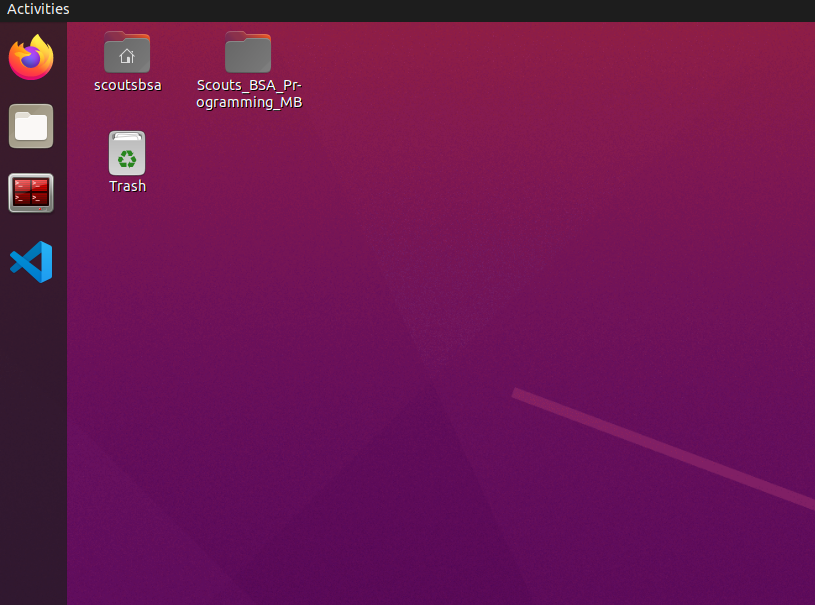
\includegraphics[width=0.8\linewidth]{./images/desktop.png}
      \caption{Desktop View}
      \label{fig:desktop_view}
    \end{figure}

    \FloatBarrier

    There are several icons on this screen.
    The bar on the left contains all of the programs necessary for the projects in this merit badge.
    The top image is the \texttt{FireFox} web-browser (like Google Chrome, Safari, or Internet Explorer).
    One icon down is the file explorer which allows you to see the files on the VM.
    Below the file explorer is the terminal which allows you to compile and execute programs (see \autoref{fig:terminal_icon}).
    Finally, is the the VS Code icon (see \autoref{fig:vs_code_icon}).
    VS Code is a text editor which allows code to be highlighted so it is easier to read.

    \begin{figure}[ht]
      \centering
      \begin{subfigure}{0.4\textwidth}
        \centering
        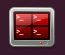
\includegraphics[width=0.5\linewidth]{./images/terminal.png}
        \caption{Terminal Icon}
        \label{fig:terminal_icon}
      \end{subfigure}
      \begin{subfigure}{0.4\textwidth}
        \centering
        
\includegraphics[width=0.5\linewidth]{./images/vs_code.png}
        \caption{VS Code Icon}
        \label{fig:vs_code_icon}
      \end{subfigure}
      \caption{Program Icons}
      \label{fig:program_icons}
    \end{figure}

    \FloatBarrier

    Now click on the terminal open it.
    This will place you in your \textit{home} folder.
    Type the \texttt{ll} command to view a list of all the files and folders in your \textit{home}.

    \begin{figure}[ht]
      \centering
      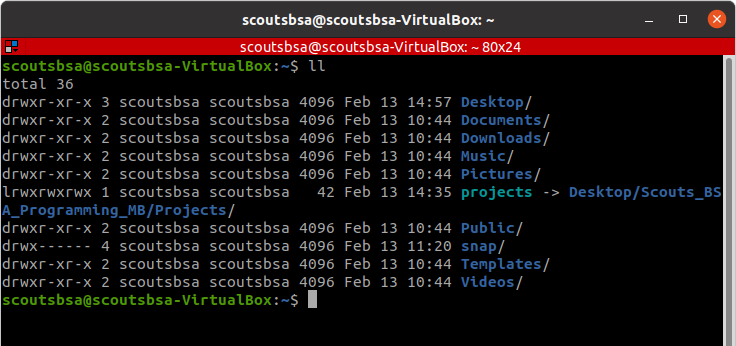
\includegraphics[width=0.8\linewidth]{./images/home_file_list.png}
      \caption{Home Directory File List}
      \label{fig:home_file_list}
    \end{figure}

    \FloatBarrier

    Notice there is a folder called projects.
    This is where all of the files you will need for your projects live.
    To get there in the terminal type \texttt{cd projects}.
    The \texttt{cd} command changes the directory you are in.
    Now find a list of the files in the projects directory.

    \begin{figure}[ht]
      \centering
      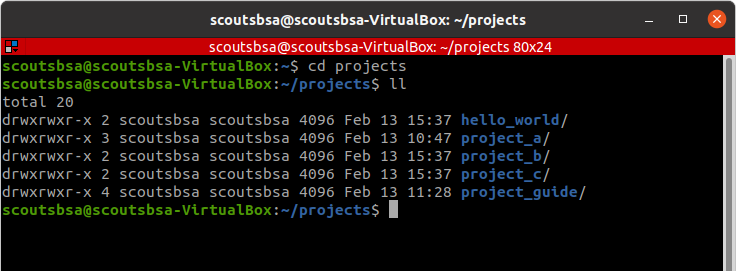
\includegraphics[width=0.8\linewidth]{./images/projects_file_list.png}
      \caption{Project Directory File List}
      \label{fig:proj_file_list}
    \end{figure}

    \FloatBarrier

    Now we want to go into the into the \textit{hello\_world} folder.
    Again use \texttt{cd} to do this.

    Once in the \textit{hello\_world} folder view the two files using \texttt{ll}.
    Notice a file called \textit{Makefile}.
    This is the file which controls how all of your projects are run.
    Use the command \texttt{make} to view what it does in this folder.

    \begin{figure}[ht]
      \centering
      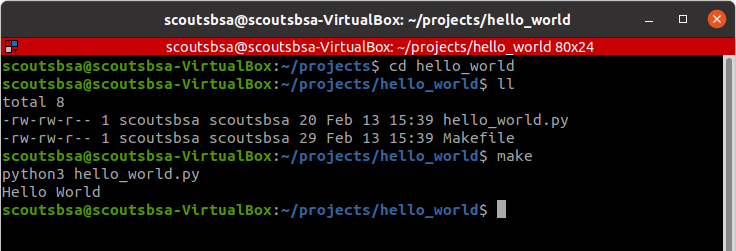
\includegraphics[width=0.8\linewidth]{./images/hello_world.png}
      \caption{Project Directory File List}
      \label{fig:hello_world_example}
    \end{figure}

    \FloatBarrier

    Now that you've seen how we are going to run our projects let's explore how we are going
      to change the code.
    Open the VS Code window by clicking on the VS Code icon on the left.
    The left hand side should contain a list of files and folders.
    At the top of this section the folder name which you are currently looking at 
      should be displayed.
    VS Code should have automatically opened to the \texttt{projects} folder.
    If not use \textit{File $\rightarrow$ Open Folder} to open the projects folder in your home directory.

    Now click the hello world folder on the left-hand bar.
    You should see the same two files we saw in the terminal.
    Click \texttt{hello\_world.py} to open the file.
    This file is extremely simple, so for now just change the "Hello World" message to another message of your choosing.
    Then rerun make in the terminal.
    You should now see your message displayed!

  \section{Next Steps}
  \label{sec:next_steps}

    Now you should be ready to go!
    Head on over to the \nameref{chap:project_a} chapter to get started.

    If you've had any troubles in this section let your councilor know before moving on.

  \chapter{Project A}
\label{chap:project_a}

  \chapter{Project B}
\label{chap:project_b}

  \chapter{Project C}
\label{chap:project_c}

\appendix

  \chapter{Developing in Windows vs Linux vs Mac}
  \label{app:dev_os}

    \section{WSL: The Best of Both Worlds?}

  \chapter{Tool Installations}
  \label{app:tool_installations}
    This appendix contains the instructions necessary to install the various tools on a variety of operating
      systems.
    Currently it is heavily lacking, but can be easily updated upon request if a scout is opting to use
      an operating system and language which are not currently listed.

    \section{JavaScript}

    \section{Python}

    \section{C++}

    \section{C}

    \section{BASIC}

    \section{Fortran}

    \section{Prolog}

    \section{SystemVerilog, Verilog, VHDL}
    \label{app:installations:HDL}

\end{document}
